% !TEX TS-program = pdfLaTeX+shellescape
% !TEX encoding = UTF-8 Unicode

\documentclass[class=beamer,tikz]{standalone}
\setbeamertemplate{navigation symbols}{} % For delete the navigation symbols
\usepackage{pgfplots}
\pgfplotsset{compat=1.17}

\begin{document}
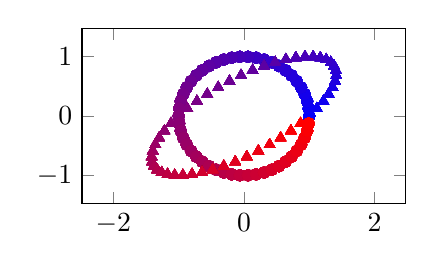
\begin{tikzpicture}[baseline]
\begin{axis}[
scale=0.6, % scale
xmin=-2.48,xmax=2.48,ymin=-1.48,ymax=1.48, % range of plot
legend style={at={(axis cs: 1,0)}, anchor=south east}, % position of legends
unit vector ratio = {1,1}, % aspect ratio
axis lines = box, % middle or box
%axis x line = bottom, % top, middle, bottom, none: axis x line* = ... removes arrow heads
%axis y line = left, % left, center, right, none: axis y line* = ... removes arrow heads
%xlabel = {$x$}, ylabel = {$y$}, % axis labels 
]
%\foreach \x in {0.,0.1,0.2,0.3,0.4,0.5,0.6,0.7,0.8,0.9,1.}
%    \node at (axis cs: )
%\draw[very thick,->,>=stealth] (axis cs:0,0) -- (axis cs:1,0.5);
%\draw[very thick,->,>=stealth] (axis cs:0,0) -- (axis cs:1.25,1.);
%\node at (axis cs: 1,0.35) {$\mathbf{v}$};
%\node at (axis cs: 1.25,1.15) {$A\mathbf{v}$};
%\addplot[black,mark=none]gnuplot{y=x};
%\addplot[black,mark=none]gnuplot{"data_bubble60h.txt" index 432};
%\addplot[magenta,mark=none]gnuplot{"data_bubble60zeta.txt" index 432};
%\legend{bubble height $h$, liquid height $\zeta$}
%\addplot+[samples = 50,domain = 0:360,scatter,only marks,scatter src=rawx]
%    ({cos(x)},{sin(x)});

\pgfmathsetmacro{\N}{50}
\foreach \k in {1,...,\N}{
    \pgfmathsetmacro{\r}{\k*2}
    \edef\temp{
        \noexpand
        \addplot[only marks,mark=*,color=red!\r!blue]
            ({cos((\k-1)*360/\N)},{sin((\k-1)*360/\N)});
        }
    \temp
    \edef\temp{
        \noexpand
        \addplot[only marks,mark=triangle*,color=red!\r!blue]
            ({cos((\k-1)*360/\N)+sin((\k-1)*360/\N)},{sin((\k-1)*360/\N)});
        }
    \temp
    }
%\foreach \k in {0,...,50}
%    \addplot+[scatter,only marks,mark=square*]
%        ({cos(\k*360/50)+1/2*sin(\k*360/50)},{sin(\k*360/50)+1/2*cos(\k*360/50)});
%\addplot+[samples = 50,domain = 0:360,scatter,only marks,scatter src=rawx]
%    ({cos(x)+1/2*sin(x)},{sin(x)+1/2*cos(x)});
\end{axis}
\end{tikzpicture}
\end{document}